\section{Introduction}
\label{sec:intro}



Graphs are an essential abstraction for a wide range of problems.  There are 
many ways to represent algorithms over graphs.  One class of methods defines
graphs in terms of matrices.  For example, we can define a graph in terms of an 
adjacency matrix where the rows and columns are labeled by the vertices and the
non-zero elements of the matrix are the edges between vertices.  

Expressing graph algorithms in the ``language of linear
algebra''~\cite{kepner2011graph} is a mature subject with multiple 
high performance graph libraries based on sparse 
linear algebra~\cite{combblas,
gadepally2015graphulo, gpi2016, sundaram2015graphmat,che2016programming}.  

A community of researchers came together to define common building
blocks for graphs expressed in the language of linear algebra.  They launched
this effort with a position paper~\cite{hpec13} in 2013 and formed the GraphBLAS
Forum~\cite{graphblas_web} to standardize the low-level building
blocks used in these graph algorithms.  After almost three years of steady work,
the GraphBLAS forum completed the
mathematical formalizations of GraphBLAS~\cite{mathgraphblas16}. With another 
one and a half years of work, the group completed the C
language binding to the GraphBLAS math spec~\cite{cspec}.

Currently there are multiple implementations of the GraphBLAS C specification.  
We have learned a great deal about how to define these operations and how to 
implement them efficiently.  We are now ready to launch the next phase of the project:
to produce a library of high level graph algorithms implemented on top of the GraphBLAS.
We call this library of algorithms \emph{LAGraph}.
Just as we launched the GraphBLAS project with a position paper, we are launching 
this next phase of the project with a position paper.  

The goals of the LAGraph effort is first and foremost to bring together the full 
range of known graph algorithms that can be constructed with the GraphBLAS.
From this collection we will be able to systematically asses the coverage of 
graph algorithms based on Linear Algebra. This will also serve
as raw material in ongoing studies of the fundamental design patterns exploited 
by linear algebra based graph algorithms. 

Initially, LAGraph is not intended to be a production-worthy library of 
high level graph algorithms.  We expect over time, however, that from the LAGraph 
effort, we will produce such a library.  Anticipating that goal, we are constructing
the library ``as if'' it was to be used by data analytics end-users; i.e. by people
who need the results from graph algorithms with little concern for how they are
implemented.  This requirement of building a library for \emph{end-users} as opposed to 
a library for \emph{graph algorithm researchers} has far reaching implications for the 
design of this software.

\begin{figure}[t]
	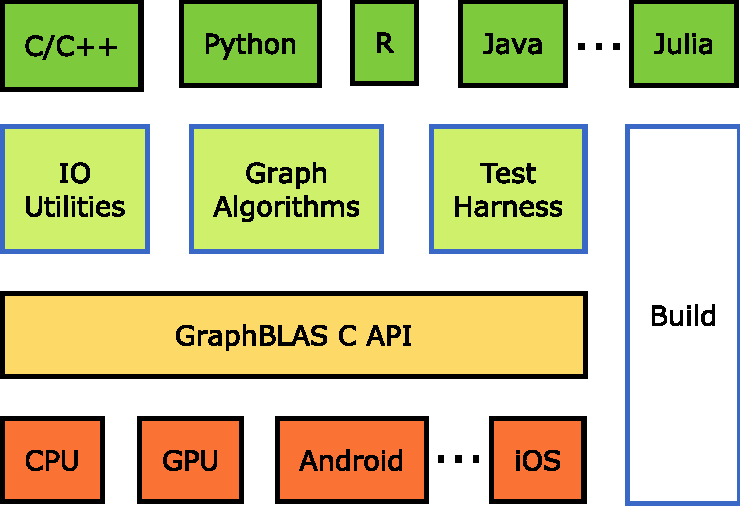
\includegraphics[width=\linewidth]{fig/lagraph}
	\label{fig:overview}
	\caption
	{\textbf{LAGraph Overview.}}
\end{figure}

We start the paper with a brief summary of the objects and operations defined in
the C specification of the GraphBLAS.  Next, we describe
the repository where we will build LAGraph.  This is important since the
purpose of a position paper is to attract a community of researchers to join the effort
which means we want people to understand how to work with and perhaps contribute 
algorithms to the repository.  We then discuss the challenges we faced in writing the 
early version LAGraph and what it suggests about future developments needed in the
GraphBLAS themselves. We close with concluding remarks.














